\documentclass[aspectratio=169,12pt]{beamer}
\usepackage{amsmath}
\usepackage{amssymb}
\usepackage[most]{tcolorbox}
\usepackage{tikz}
\usepackage{graphicx}
\usepackage[sfdefault,lf]{FiraSans}
\renewcommand{\familydefault}{\sfdefault}
\setlength{\parindent}{0pt}
\everymath{\displaystyle}

\setbeamertemplate{navigation symbols}{}
\setbeamertemplate{footline}{}
\setbeamertemplate{headline}{}

\definecolor{mmpageWhite}{HTML}{FCFBF7}
\definecolor{mmtanSoft}{HTML}{F7F5EF}
\definecolor{mmgreenDeep}{HTML}{244B2C}
\definecolor{mmgreenLeaf}{HTML}{5D8A56}
\definecolor{mmgreenSoft}{HTML}{E4EFD9}
\definecolor{mmtext}{HTML}{163221}

\setbeamercolor{background canvas}{bg=mmpageWhite}
\setbeamercolor{normal text}{fg=mmtext,bg=mmpageWhite}

\newtcolorbox{MMProblemCard}[1][]{enhanced,breakable=false,colback=white,colframe=black,boxrule=1.5pt,arc=8pt,left=5pt,right=5pt,top=4pt,bottom=4pt,before skip=0pt,after skip=0pt,height=0.245\textheight,valign=top,#1}
\newcommand{\KoruIcon}{\raisebox{-0.2em}{
\includegraphics[height=1.05em]{../../SITE/header-logo.png}}}
\newcommand{\ScaffoldIcons}[1]{\ifcase#1\or \KoruIcon\or \KoruIcon\hspace{0.22em}\KoruIcon\or \KoruIcon\hspace{0.22em}\KoruIcon\hspace{0.22em}\KoruIcon\fi}
\newcommand{\WorksheetTitle}[2]{%
  {\colorbox{mmtanSoft}{\parbox[c][2.0em][c]{0.975\linewidth}{%
    \hspace{0.25em}{\Large\bfseries\textcolor{mmgreenDeep}{#1}\hfill\ScaffoldIcons{#2}}}}
  \par\vspace{0.08em}{\color{mmgreenLeaf}\rule{\linewidth}{2.0pt}}\par\vspace{0.04em}}
}
\newcommand{\MMProblem}[2]{\begin{MMProblemCard}\raggedright\small\textbf{#1.} #2\par\end{MMProblemCard}}

\setbeamertemplate{background}{
 \begin{tikzpicture}[remember picture,overlay]
 \draw[black,line width=1.5pt,rounded corners=10pt]
 ([xshift=0.45cm,yshift=-0.45cm]current page.north west)
 rectangle
 ([xshift=-0.45cm,yshift=0.45cm]current page.south east);
 \end{tikzpicture}
}

% Default worksheet generation rules:
% use notes-style beamer pages
% use bordered cards for individual problems
% target 9 problems per frame in a 3x3 grid
% target 3 frames per scaffold by default where content allows

\begin{document}\begin{frame}[t]
\WorksheetTitle{Start Tasks}
\vspace{-0.18em}
\begin{columns}[T,onlytextwidth]
\begin{column}{0.32\textwidth}\MMProblem{1}{Find the volume of this cube.\\[0.4em]
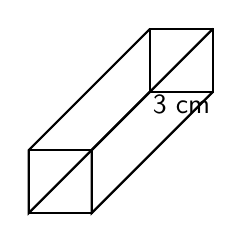
\begin{tikzpicture}[x=0.2cm,y=0.2cm,baseline=(current bounding box.center)]
  \draw[thick] (0,0,0) -- (4,0,0) -- (4,4,0) -- (0,4,0) -- cycle;
  \draw[thick] (0,0,0) -- (0,0,4) -- (0,4,4) -- (0,4,0);
  \draw[thick] (4,0,0) -- (4,0,4) -- (4,4,4) -- (4,4,0);
  \draw[thick] (0,0,4) -- (4,0,4) -- (4,4,4) -- (0,4,4) -- cycle;
  \draw[dashed] (0,0,0) -- (0,0,4);
  \draw[dashed] (4,0,0) -- (4,0,4);
  \draw[dashed] (0,4,0) -- (0,4,4);
  \draw[dashed] (4,4,0) -- (4,4,4);
  \node at (2,-0.8) {3 cm};
\end{tikzpicture}}\end{column}
\begin{column}{0.32\textwidth}\MMProblem{2}{Find the volume of this cube.\\[0.4em]
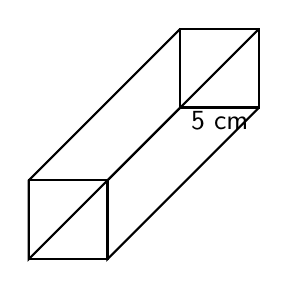
\begin{tikzpicture}[x=0.2cm,y=0.2cm,baseline=(current bounding box.center)]
  \draw[thick] (0,0,0) -- (5,0,0) -- (5,5,0) -- (0,5,0) -- cycle;
  \draw[thick] (0,0,0) -- (0,0,5) -- (0,5,5) -- (0,5,0);
  \draw[thick] (5,0,0) -- (5,0,5) -- (5,5,5) -- (5,5,0);
  \draw[thick] (0,0,5) -- (5,0,5) -- (5,5,5) -- (0,5,5) -- cycle;
  \draw[dashed] (0,0,0) -- (0,0,5);
  \draw[dashed] (5,0,0) -- (5,0,5);
  \draw[dashed] (0,5,0) -- (0,5,5);
  \draw[dashed] (5,5,0) -- (5,5,5);
  \node at (2.5,-0.8) {5 cm};
\end{tikzpicture}}\end{column}
\begin{column}{0.32\textwidth}\MMProblem{3}{Find the volume of this cuboid.\\[0.4em]
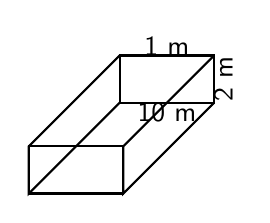
\begin{tikzpicture}[x=0.15cm,y=0.15cm,baseline=(current bounding box.center)]
  \draw[thick] (0,0,0) -- (8,0,0) -- (8,4,0) -- (0,4,0) -- cycle;
  \draw[thick] (0,0,0) -- (0,0,3) -- (0,4,3) -- (0,4,0);
  \draw[thick] (8,0,0) -- (8,0,3) -- (8,4,3) -- (8,4,0);
  \draw[thick] (0,0,3) -- (8,0,3) -- (8,4,3) -- (0,4,3) -- cycle;
  \draw[dashed] (0,0,0) -- (0,0,3);
  \draw[dashed] (8,0,0) -- (8,0,3);
  \draw[dashed] (0,4,0) -- (0,4,3);
  \draw[dashed] (8,4,0) -- (8,4,3);
  \node at (4,-0.8) {10 m};
  \node[rotate=90] at (8.8,2) {2 m};
  \node at (4,4.8) {1 m};
\end{tikzpicture}}\end{column}
\end{columns}
\vspace{0.45em}
\begin{columns}[T,onlytextwidth]
\begin{column}{0.32\textwidth}\MMProblem{4}{Find the volume of this cuboid.\\[0.4em]
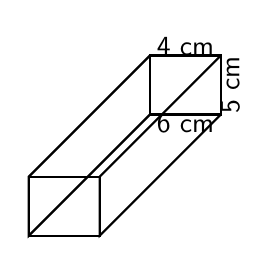
\begin{tikzpicture}[x=0.15cm,y=0.15cm,baseline=(current bounding box.center)]
  \draw[thick] (0,0,0) -- (6,0,0) -- (6,5,0) -- (0,5,0) -- cycle;
  \draw[thick] (0,0,0) -- (0,0,4) -- (0,5,4) -- (0,5,0);
  \draw[thick] (6,0,0) -- (6,0,4) -- (6,5,4) -- (6,5,0);
  \draw[thick] (0,0,4) -- (6,0,4) -- (6,5,4) -- (0,5,4) -- cycle;
  \draw[dashed] (0,0,0) -- (0,0,4);
  \draw[dashed] (6,0,0) -- (6,0,4);
  \draw[dashed] (0,5,0) -- (0,5,4);
  \draw[dashed] (6,5,0) -- (6,5,4);
  \node at (3,-0.8) {6 cm};
  \node[rotate=90] at (6.8,2.5) {5 cm};
  \node at (3,5.8) {4 cm};
\end{tikzpicture}}\end{column}
\begin{column}{0.32\textwidth}\MMProblem{5}{A cube has side length 4 m. What is its volume?}\end{column}
\begin{column}{0.32\textwidth}\MMProblem{6}{A cuboid is 12 cm long, 3 cm wide, and 2 cm high. What is its volume?}\end{column}
\end{columns}
\vspace{0.45em}
\begin{columns}[T,onlytextwidth]
\begin{column}{0.32\textwidth}\MMProblem{7}{A cube has side length 7 cm. What is its volume?}\end{column}
\begin{column}{0.32\textwidth}\MMProblem{8}{A cuboid is 9 m long, 2 m wide, and 1 m high. What is its volume?}\end{column}
\begin{column}{0.32\textwidth}\MMProblem{9}{A cube has side length 2.5 cm. What is its volume?}\end{column}
\end{columns}
\end{frame}
\begin{frame}[t]
\WorksheetTitle{Start Tasks}
\vspace{-0.18em}
\begin{columns}[T,onlytextwidth]
\begin{column}{0.32\textwidth}\MMProblem{1}{A cuboid is 15 mm long, 4 mm wide, and 3 mm high. What is its volume?}\end{column}
\begin{column}{0.32\textwidth}\MMProblem{2}{How many cubic centimetres are in 1 cubic metre?}\end{column}
\begin{column}{0.32\textwidth}\MMProblem{3}{How many cubic millimetres are in 1 cubic centimetre?}\end{column}
\end{columns}
\vspace{0.45em}
\begin{columns}[T,onlytextwidth]
\begin{column}{0.32\textwidth}\MMProblem{4}{A cube has volume 27 cm\mbox{$^3$}. What is its side length?}\end{column}
\begin{column}{0.32\textwidth}\MMProblem{5}{A cuboid has volume 60 m\mbox{$^3$}, length 5 m, and width 3 m. What is its height?}\end{column}
\begin{column}{0.32\textwidth}\MMProblem{6}{A cube has volume 64 mm\mbox{$^3$}. What is its side length?}\end{column}
\end{columns}
\vspace{0.45em}
\begin{columns}[T,onlytextwidth]
\begin{column}{0.32\textwidth}\MMProblem{7}{A cuboid has volume 48 cm\mbox{$^3$}, length 6 cm, and height 2 cm. What is its width?}\end{column}
\begin{column}{0.32\textwidth}\MMProblem{8}{}\end{column}
\begin{column}{0.32\textwidth}\MMProblem{9}{}\end{column}
\end{columns}
\end{frame}
\end{document}
